\documentclass{article}
\usepackage{tikz}

\begin{document}

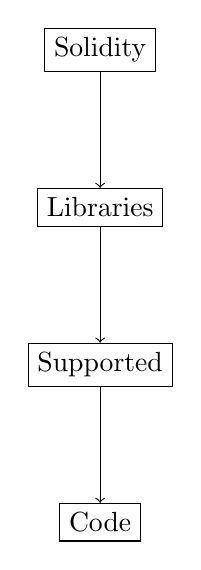
\begin{tikzpicture}[node distance=2cm]
    \node (solidity) [draw, rectangle] {Solidity};
    \node (libraries) [draw, rectangle, below of=solidity] {Libraries};
    \node (supported) [draw, rectangle, below of=libraries] {Supported};
    \node (code) [draw, rectangle, below of=supported] {Code};
    
    \draw[->] (solidity) -- (libraries);
    \draw[->] (libraries) -- (supported);
    \draw[->] (supported) -- (code);
\end{tikzpicture}

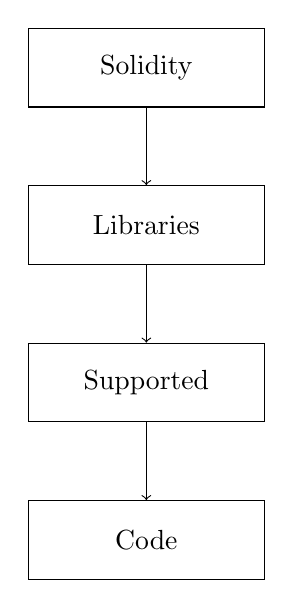
\begin{tikzpicture}[node distance=2cm, every node/.style={draw, rectangle, minimum width=3cm, minimum height=1cm}]
    \node (solidity) {Solidity};
    \node (libraries) [below of=solidity] {Libraries};
    \node (supported) [below of=libraries] {Supported};
    \node (code) [below of=supported] {Code};
    
    \draw[->] (solidity) -- (libraries);
    \draw[->] (libraries) -- (supported);
    \draw[->] (supported) -- (code);
\end{tikzpicture}

\end{document}